
\chapter{Introduction - Project Context}
\label{ch:introduction}
\pagestyle{headings}

\section{Project context}
\label{sec:introduction-context}

\subsection{General Context}
\label{subsec:introduction-general-context}
With the increase of internet speed across the globe, possible among others to the appearance of 5G networks and, in
the near future, to the SpaceX Starlink network, it is now possible to stream increasingly larger data across the
internet. \
According to .., \ % todo: insert reference https://www.speedtest.net/global-index#mobile
the global mobile internet speed was of about 31Mbps for download and 11.88Mbps for upload. \
Although these values are still pretty low, they are bound to improve in the near future.
The highest values were achieved using 4G LTE and 4G LTE-A networks.

\begin{table}[ht]
    \caption{Average internet speed}
    \centering
    \begin{tabular}{|c|c|c|}
        \hline\hline
        Rank & Country & Download speed $[Mbps]$ \\ $[0.5ex]$
        \hline
        1 & South Korea & 117.79 \\
        2 & Qatar & 77.07  \\
        3 & Norway & 72.80 \\
        4 & UAE & 69.72 \\
        5 & Australia & 68.87 \\
        6 & Canada & 67.57 \\
        7 & Netherlands & 62.86 \\
        8 & Croatia & 59.83 \\
        9 & China & 58.33 \\
        10 & Switzerland & 57.09 \\
        40 & Romania & 37.76
    \end{tabular}
    \label{table:internetSpeed}
\end{table}

% todo: mention ml/deep learning

\subsection{5G}
\label{subsec:5g}
According to ..\ % todo: quote https://www.telekom.com/en/company/details/5g-speed-is-data-transmission-in-real-time-544498
5G internet speeds should reach speeds of about 10Gbps, enough to stream video-audio in real time.
However, according to .. \ % todo: quote https://www.forbes.com/sites/bobodonnell/2019/11/22/real-world-5g-speeds/#3ec794804f96
and ..,\ % todo: quote https://5g.co.uk/guides/how-fast-is-5g/
such speeds cannot be reached with the current infrastructure, with download speeds averaging at about 130Mbps-240Mbps, \
with peaks at about 600Mbps.
However, certain variants have reached peaks of 1.8 Gbps (using mmWave 5G services) and event 1Tbps in controlled \
test environments.

It must be noted that these are only the early days of 5G networks, and that in the coming years these speeds are \
bound to improve.

According to .. \ % todo: quote https://web.archive.org/web/20190419231844/http://www.5gamericas.org/files/5115/4169/8314/5G_Americas_URLLLC_White_Paper_Final_11.8.pdf , https://en.wikipedia.org/wiki/5G
possible use cases for 5G networks include but are not limited to  Smart Factories (industrial control, robot control),\
 healthcare (remote diagnosis and surgery), entertainment (immersive entertainment, online gaming), transport \
industry (driver assistance, enhanced safety, autonomous driving, traffic management), energy sector (smart energy, \
smart grid).


\subsection{Satellite internet}
\label{subsec:satellite-internet}
As mentioned in .., \ % todo: quote https://www.forbes.com/sites/bobodonnell/2019/11/22/real-world-5g-speeds/#3ec794804f96
for 5G, the radio wave internet speed is inversely proportional to the distance covered. \
This means that regular 5G high speed internet will probably be limited to regions densely and medium populated and \
to research outposts because of infrastructure costs. \
A valid alternative for sparsely populated areas would be satellite internet. \
Several US companies have already begun taking steps towards a commercial solution. \
The most notable player is SpaceX with its project, Starlink, a network of several dozen thousands satellites in lower \
Earth orbit, in the range of 350\-550 km from Earth, as opposed to the average altitude of \
1000+ km for satellites in lower earth orbit. \
According to .. , % todo: quote https://www.pcmag.com/news/371511/spacexs-satellite-internet-plans-for-mid-2020-launch-in-the
the desired average speed is about 1Gbps. \
 .. % todo: quote https://spacenews.com/spacex-launches-second-batch-of-starlink-broadband-satellites/
mentions that tests with the US military achieved peak speeds of around 610 Mbps, while the network isn't fully \
functional yet, with thousands of satellites still to be sent to space. \
The official \href{https://www.starlink.com/}{Starlink} website it expects to reach coverage for northern US and \
Canada by 2020, and for the rest of the world by 2021.\
Other companies, including Amazon and OneWeb, have started work on deploying their own internet satellite network.

\subsection{Motivation}
\label{subsec:introduction-motivation}
With the rise of 5G internet and satellite-based internet, it will be increasingly easier to stream real-time data \
from one place in the world to another place on the opposite side. \
One use case for this increase in speed is the development of commercial drones controlled remotely over the internet.\
With 5G's speed, bandwidth and latency, it will be possible for a robot to transmit in virtually real-time audio-video \
data to a remote operator and to receive control commands from that operator.

\begin{figure}[ht]
    \label{fig:overview1}
    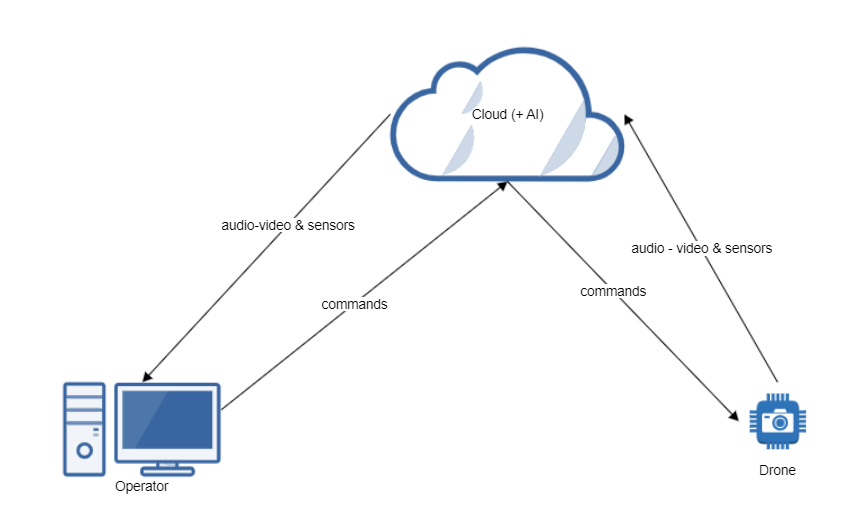
\includegraphics[width=15cm, height=10cm, keepaspectratio]{img/overview1.PNG}
    \caption{High Level Overview}
\end{figure}

This use case can be extended to autonomous robots. \
Instead of adding considerable computation capabilities to a robot (CPU, memory, GPU) os that it can run an AI, the \
robot could be fitted with minimal hardware designed only to transmit audio-video and receive commands from an AI that \
runs in the cloud. \
This way, if any malfunction occurs on the robot, the equipment could be easily replaced with lower costs because the \
equipment used was a lot cheaper than it would have been if hardware had to run the AI . \
Another option would be to use dedicated hardware that puts an emphasis on durability and can properly function in \
a wide range of conditions (rain, extreme low/high temperatures). \
Additionally, this type of setup would also use less energy in order to run, thus extending battery life and allowing \
higher autonomy.


